%---------- Inleiding ---------------------------------------------------------

\section{Introductie}%
\label{sec:introductie}

De bachelorproef zal zich focussen op de evoluerende complexiteit van moderne bedrijfsapplicaties en de architecturale benaderingen die worden ingezet om aan deze groeiende behoeften te voldoen. Het kernthema van mijn onderzoek betreft de keuze tussen een monolithische architectuur en een microservices architectuur bij de ontwikkeling van bedrijfsapplicaties. Deze keuze wordt steeds relevanter vanwege de voortdurende toename en verandering van de complexiteit waarmee ondernemingen te maken hebben. Bedrijven overwegen vaak om de stabiliteit van een monolithische softwarearchitectuur los te laten en te opteren voor een servicegerichte architectuur. Het onderzoek is gedreven door de noodzaak van flexibiliteit in softwarearchitecturen, en daarom wordt de beweging van veel bedrijven om over te stappen van een monolithische naar een servicegerichte aanpak nauwgezet onderzocht. Het centrale thema van de bachelorproef is de vergelijking tussen beide architecturen, waarbij specifieke aandacht wordt besteed aan de voor- en nadelen van elk. De verschuiving naar een servicegerichte benadering wordt verder onderzocht met als doel richtlijnen te ontwikkelen voor bedrijven die deze overgang overwegen. Dit onderzoek wordt concreet toegepast in een casestudy over software in een dierenkliniek, waarmee praktische inzichten worden verkregen die relevant zijn voor de bredere context van bedrijfsapplicatieontwikkeling.

In het kader van deze studie zal ik me specifiek richten op een dierenkliniekapplicatie, die zal eerst opgezet worden als een monolithische architectuur met behulp van Spring Boot. Deze applicatie omvat diverse functionaliteiten, zoals het beheer van klanten, dieren en artsen, het maken van afspraken, het registreren van prestaties, het aanmaken en verzenden van facturen, en het volgen van betalingen.

Het onderzoek heeft als doel inzicht te bieden in de mogelijkheden van schaalbaarheid en prestatieverbetering door de overstap naar een microservices architectuur in combinatie met een servicemesh. Hierbij zal ik de functionaliteiten van de applicatie opdelen in verschillende microservices, zoals CRM, beheer van afspraken, beheer van prestaties, facturatie en betalingen. Deze microservices zullen vervolgens worden beheerd en met elkaar communiceren via een servicemesh.

Om dit doel te bereiken, zal ik me richten op de volgende aspecten:

Kaderen van het thema: Het onderzoek zal de overstap van een monolithische naar een microservices architectuur in de context van bedrijfsapplicaties belichten, met bijzondere aandacht voor de dierenkliniekapplicatie.

Doelgroep: De doelgroep van dit onderzoek zijn ontwikkelaars, architecten en besluitvormers die betrokken zijn bij de bouw en evolutie van bedrijfsapplicaties.

Probleemstelling en (centrale) onderzoeksvraag: De huidige monolithische architectuur van de dierenkliniekapplicatie roept vragen op over schaalbaarheid en prestaties. De centrale onderzoeksvraag luidt: "Hoe kan de dierenkliniekapplicatie profiteren van een microservices architectuur in combinatie met een servicemesh om schaalbaarheid en prestaties te verbeteren?"

Onderzoeksdoelstelling: Het onderzoek streeft ernaar inzicht te verschaffen in de architecturale overwegingen en best practices bij het gebruik van een servicemesh voor schaalbaarheid en prestatieverbetering in bedrijfsapplicaties, met de dierenkliniekapplicatie als specifieke case study.

In de vervolgstappen van dit onderzoeksvoorstel zal ik dieper ingaan op relevante literatuur, de toegepaste methodologie, en de verwachte resultaten en conclusies die ik hoop te verkrijgen.
%---------- Stand van zaken ---------------------------------------------------

\section{State-of-the-art}%
\label{sec:state-of-the-art}

We kunnen de vergelijking maken  tussen monolithische en microservices architectuur. Een monolithische architectuur bestaat uit één codebase met alle functionaliteit, terwijl een  microservices architectuur gebruik maakt van onafhankelijke services. Microservices bieden flexibiliteit en schaalbaarheid, maar brengen ook complexiteit met zich mee, zoals service discovery en monitoring. De juiste architectuurkeuze hangt af van de behoeften en complexiteit van het project.

Deze adoptie van microservices architectuur heeft geleid tot de opkomst van servicemeshes als een mechanisme voor het beheren van de communicatie en interactie tussen de verschillende services binnen een applicatie. Een servicemesh is een abstractielaag die een reeks functies biedt, zoals load balancing, service discovery, monitoring en beveiliging, die essentieel zijn voor het schalen en beheren van microservices.

Een belangrijke architecturale overweging bij het gebruik van een servicemesh is service discovery. In tegenstelling tot een monolithische architectuur, waarbij functionaliteiten vaak hardgecodeerde afhankelijkheden hebben, maakt een servicemesh gebruik van dynamische service discovery. Dit stelt services in staat om automatisch nieuwe services te ontdekken en ermee te communiceren zonder handmatige configuratiewijzigingen. Een voorbeeld van een servicemesh implementatie die service discovery mogelijk maakt, is Istio \autocite{Morgan2021}.

Een andere belangrijk aspect is load balancing. Een servicemesh verdeelt het verkeer gelijkmatig over de beschikbare service instances, waardoor de prestaties worden geoptimaliseerd, de belasting op afzonderlijke instances onder controle blijft en er ad hoc extra instances kunnen opgespind worden. Dit is vooral nuttig in bedrijfsapplicaties waar veel services parallel moeten worden geschaald om aan de vraag te voldoen \autocite{Ciobotaru2020}.

Monitoring en tracing van service traffic zijn ook cruciale aspecten bij het gebruik van een servicemesh. Door het instrumenteren van services met monitoring- en tracingfunctionaliteit, kan een servicemesh gedetailleerd inzicht bieden in de prestaties en het gedrag van services. Dit is met name waardevol in bedrijfsapplicaties waar de complexiteit van de interacties tussen services kan leiden tot moeilijkheden bij het identificeren en oplossen van problemen \autocite{Ciobotaru2021}.

Servicemeshes verhogen de weerbaarheid door het implementeren van verschillende resilience patterns. Hierdoor kan tijdelijke onbeschikbaarheid of overbelasting van services opgevangen worden.

% Voor literatuurverwijzingen zijn er twee belangrijke commando's:
% \autocite{KEY} => (Auteur, jaartal) Gebruik dit als de naam van de auteur
%   geen onderdeel is van de zin.
% \textcite{KEY} => Auteur (jaartal)  Gebruik dit als de auteursnaam wel een
%   functie heeft in de zin (bv. ``Uit onderzoek door Doll & Hill (1954) bleek
%   ...'')


%---------- Methodologie ------------------------------------------------------
\section{Methodologie}%
\label{sec:methodologie}

Plan van aanpak
\begin{itemize}
	
	\item Fase 1: Literatuuronderzoek en probleemdefinitie (Week 1-2)
	\begin{itemize}
		\item Doelstelling: Een grondig begrip ontwikkelen van servicemesh, schaalbaarheid en prestatieproblemen in bedrijfsapplicaties en de architecturale overwegingen en best practices bij het implementeren van een servicemesh identificeren.
		\item Aanpak:
		\begin{itemize}
			\item Uitvoeren van een literatuuronderzoek naar servicemesh technologieën, schaalbaarheid, prestatieproblemen en best practices voor bedrijfsapplicaties.
			\item Identificeren van de belangrijkste architecturale verschillen tussen servicemesh- en monolithische architecturen.
			\item Analyseren van casestudies en praktijkvoorbeelden om inzicht te krijgen in de voordelen en uitdagingen van het gebruik van servicemesh voor schaalbaarheid en prestatieverbetering.
		\end{itemize}        
		\item Resultaat, deliverable(s): Een gedetailleerd overzicht kunnen geven van de concepten en technologieën met betrekking tot servicemesh, schaalbaarheid en prestatieverbetering
	\end{itemize}            
	\item Fase 2: Architecturale overwegingen en best practices identificeren (Week 3-4)
	\begin{itemize}
		\item Doelstelling De belangrijkste architecturale overwegingen en best practices identificeren die van toepassing zijn op het implementeren van een servicemesh voor schaalbaarheid en prestaties in bedrijfsapplicaties.
		\item Aanpak: 
		\begin{itemize}        
			\item Analyseren van de literatuur en case studies om patronen en gemeenschappelijke elementen te identificeren in de implementatie van servicemesh architecturen.
			\item Analyseren van casestudies en praktijkvoorbeelden om inzicht te krijgen in de voordelen en uitdagingen van het gebruik van servicemesh voor schaalbaarheid en prestatieverbetering.
		\end{itemize}            
		\item Resultaat, deliverable(s): Een lijst met belangrijke architecturale overwegingen en best practices voor het implementeren van een servicemesh in bedrijfsapplicaties en een samenvatting van de verschillen tussen servicemesh en monolithische architecturen met betrekking tot schaalbaarheid en prestatieverbetering.
	\end{itemize}
	\item Fase 3: Casus Implementatie (Week 5-8)
	\begin{itemize}
		\item Doelstelling: het implementeren van zowel de monolithische applicatie als de microservices, met servicemesh implementatie, voor de functionaliteiten van de dierenkliniek \autocite{RameshMF2018}. 
		
		\item Aanpak:
		\begin{itemize}
			\item Opzetten van de spring-boot applicatie. Verder bouwen bestaande free ware git applicatie.
			\item Opzetten van een omgeving voor de implementatie van de servicemesh.
			\item Implementeren van de servicemesh en de microservices.
			\item Uitvoeren van tests en metingen om de schaalbaarheid en prestatieverbetering te beoordelen.
		\end{itemize}   
		\item Resultaat, deliverable(s): Een experimentele implementatie van een servicemesh en een evaluatie van de architecturale overwegingen en best practices.
	\end{itemize}  
	\item Fase 4: Vergelijkende analyse en conclusies (Week 9-11)
	\begin{itemize} 
		\item Doelstelling: Een vergelijkende analyse uitvoeren tussen de servicemesh architectuur en de monolithische architectuur om de verschillen in schaalbaarheid, prestaties en andere relevante aspecten te begrijpen. Op basis hiervan conclusies trekken en aanbevelingen doen.
		\item Aanpak:
		\begin{itemize} 
			\item Verzamelen van gegevens en resultaten van eerdere fasen, inclusief literatuuronderzoek, casestudies en experimentele implementatie.
			\item Analyseren van de verzamelde gegevens om de verschillen tussen servicemesh en monolithische architecturen te identificeren, met betrekking tot schaalbaarheid, prestaties, onderhoud, flexibiliteit ...
			\item Trekken van conclusies op basis van de analyse en het formuleren van aanbevelingen voor de toepassing van servicemesh in bedrijfsapplicaties.
		\end{itemize}     
		\item Resultaat, deliverable(s):  Een vergelijkende analyse tussen servicemesh en monolithische architecturen, inclusief conclusies en aanbevelingen voor het gebruik van servicemesh in bedrijfsapplicaties.
	\end{itemize}   
	\item Fase 5: Afronding (Week 12-13)
	\begin{itemize} 
		\item Doelstelling: Het onderzoeksvoorstel afronden.
		\item Aanpak:
		\begin{itemize} 
			\item Samenstellen en schrijven van het eindrapport van de bachelorproef.
			\item Nakijken, herzien en redigeren van het rapport.
			\item Voorbereiden en indienen van het rapport.
		\end{itemize}     
		\item Resultaat, deliverable(s): Eindrapport van de bachelorproef.  
	\end{itemize}
\end{itemize}

Gedetailleerde flowchart (\ref{fig:flowchart}) en gantt-chart (\ref{fig:gantt}) vind je onderaan terug.


\section{Verwachte resultaten}%
\label{sec:verwachte-resultaten}

Op basis van het literatuuronderzoek vermoed ik dat het gebruik van een servicemesh een positieve impact zal hebben op de schaalbaarheid en prestatiesvan bedrijfsapplicaties. Het biedt de nodige abstractielaag en functionaliteiten om de complexe communicatie en interactie tussen microservices te beheren. Hoewel er altijd alternatieve mogelijkheden en verrassende resultaten kunnen zijn, lijkt het gebruik van een servicemesh zoals Istio een veelgebruikte en geschikte keuze te zijn op basis van de beschikbare literatuur.

%---------- Verwachte resultaten ----------------------------------------------
\section{Verwacht resultaat, conclusie}%
\label{sec:verwachte_resultaten}

Ik vermoed dat de impact van het gebruik van een servicemesh in bedrijfsapplicaties significant kan zijn. Het lijkt erop dat het gebruik van een servicemesh de mogelijkheid biedt om microservices op een schaalbare en onderhoudbare manier te beheren, wat kan resulteren in verbeterde prestaties, betere schaalbaarheid en een hogere flexibiliteit.

Er moet echter rekening worden gehouden met enkele beperkingen. Het implementeren van een servicemesh vereist waarschijnlijk een leercurve en investering in het begrijpen en toepassen van de juiste architecturale overwegingen en best practices. Daarnaast kan het beheer van een servicemesh complex zijn en extra infrastructuurkosten met zich meebrengen.

Om deze vermoedens verder te onderzoeken, zou het interessant zijn om de impact van servicemeshes in verschillende scenario's en bedrijfsomgevingen nader te onderzoeken. Het zou ook de moeite waard zijn om te onderzoeken hoe servicemeshes geoptimaliseerd kunnen worden voor specifieke gebruiksscenario's en welke aanpassingen nodig zijn om de prestaties verder te verbeteren.

Ten slotte vermoed ik dat de implementatie van een servicemesh in bedrijfsapplicaties aanzienlijke voordelen kan bieden op het gebied van schaalbaarheid, beschikaarheid, vindbaarheid en prestaties, mits de juiste architecturale overwegingen en best practices worden gevolgd. Het is weliswaar belangrijk om rekening te houden met de beperkingen en de specifieke behoeften van de applicatie en de bedrijfsdoelstellingen.

\begin{figure*}[t]   
	\centering   
	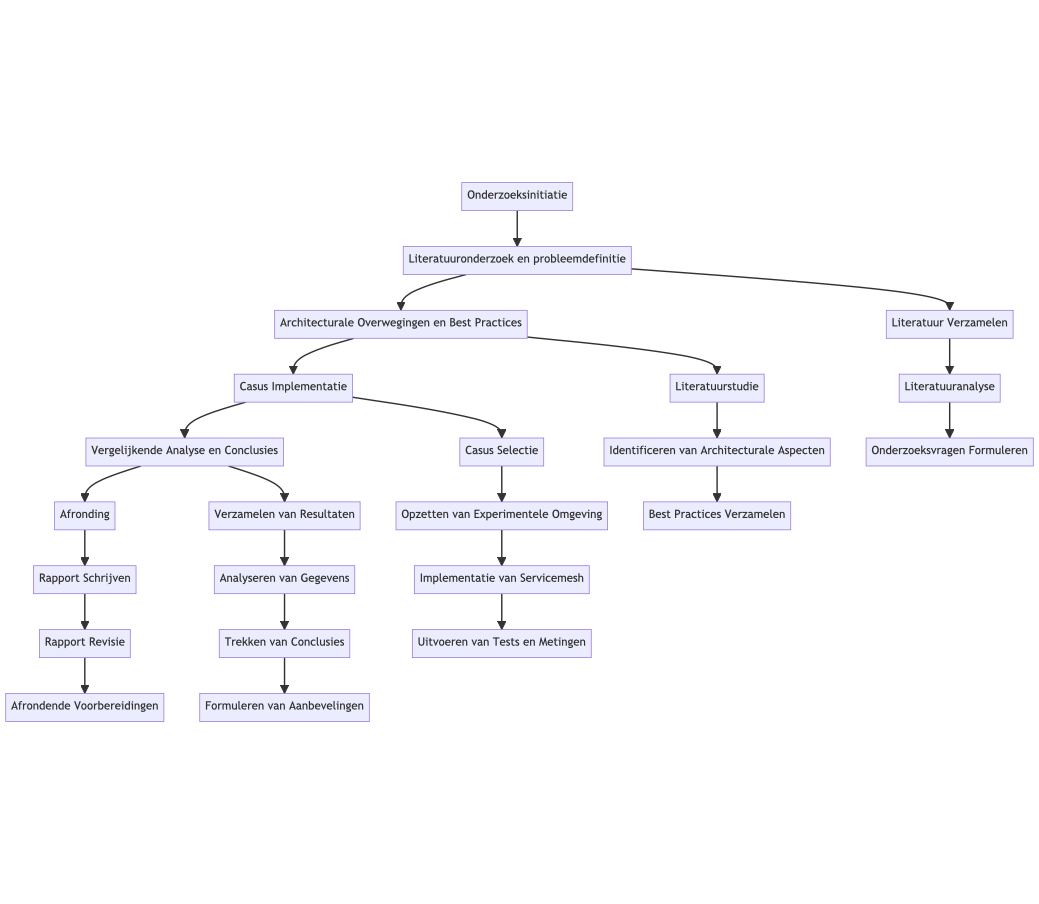
\includegraphics[width = \textwidth]{Flowchart.png}  
	\caption{Flow chart}
	\label{fig:flowchart}				 
\end{figure*} 
\begin{figure*}[t]   
	\centering   
	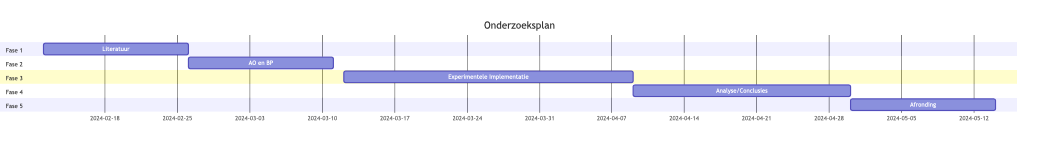
\includegraphics[width = \textwidth]{Gantt.png}   
	\caption{Gantt chart}	
	\label{fig:gantt}	
\end{figure*}